\subsection{Motor modelling}
A model of a motor consist of both a mechanical and an electrical section, due to the electrical current, $i_a(t)$, which is converted to a rotational force called torque, $\tau_m$. Therefore a model of the mechanical and the electrical system should be produced. The mechanical model from the motor will provide what the motors contributions to the drivetrain is, see \secref{DriveTrain}, and the electrical model will provide the motors torque.

\subsubsection{Mechanical model}



\begin{figure}[H]
	\setcounter{subfigure}{0}
	\centering
	\begin{subfigure}{.45\textwidth}
		\centering
		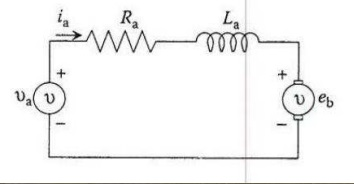
\includegraphics[width=\linewidth]{figures/MotorElektrikDiagram.jpg}
		\caption{Electric diagram of the motor}
		\label{fig:MotorElectric}
	\end{subfigure}
	\hfill
	\begin{subfigure}{.45\textwidth}
		\centering
		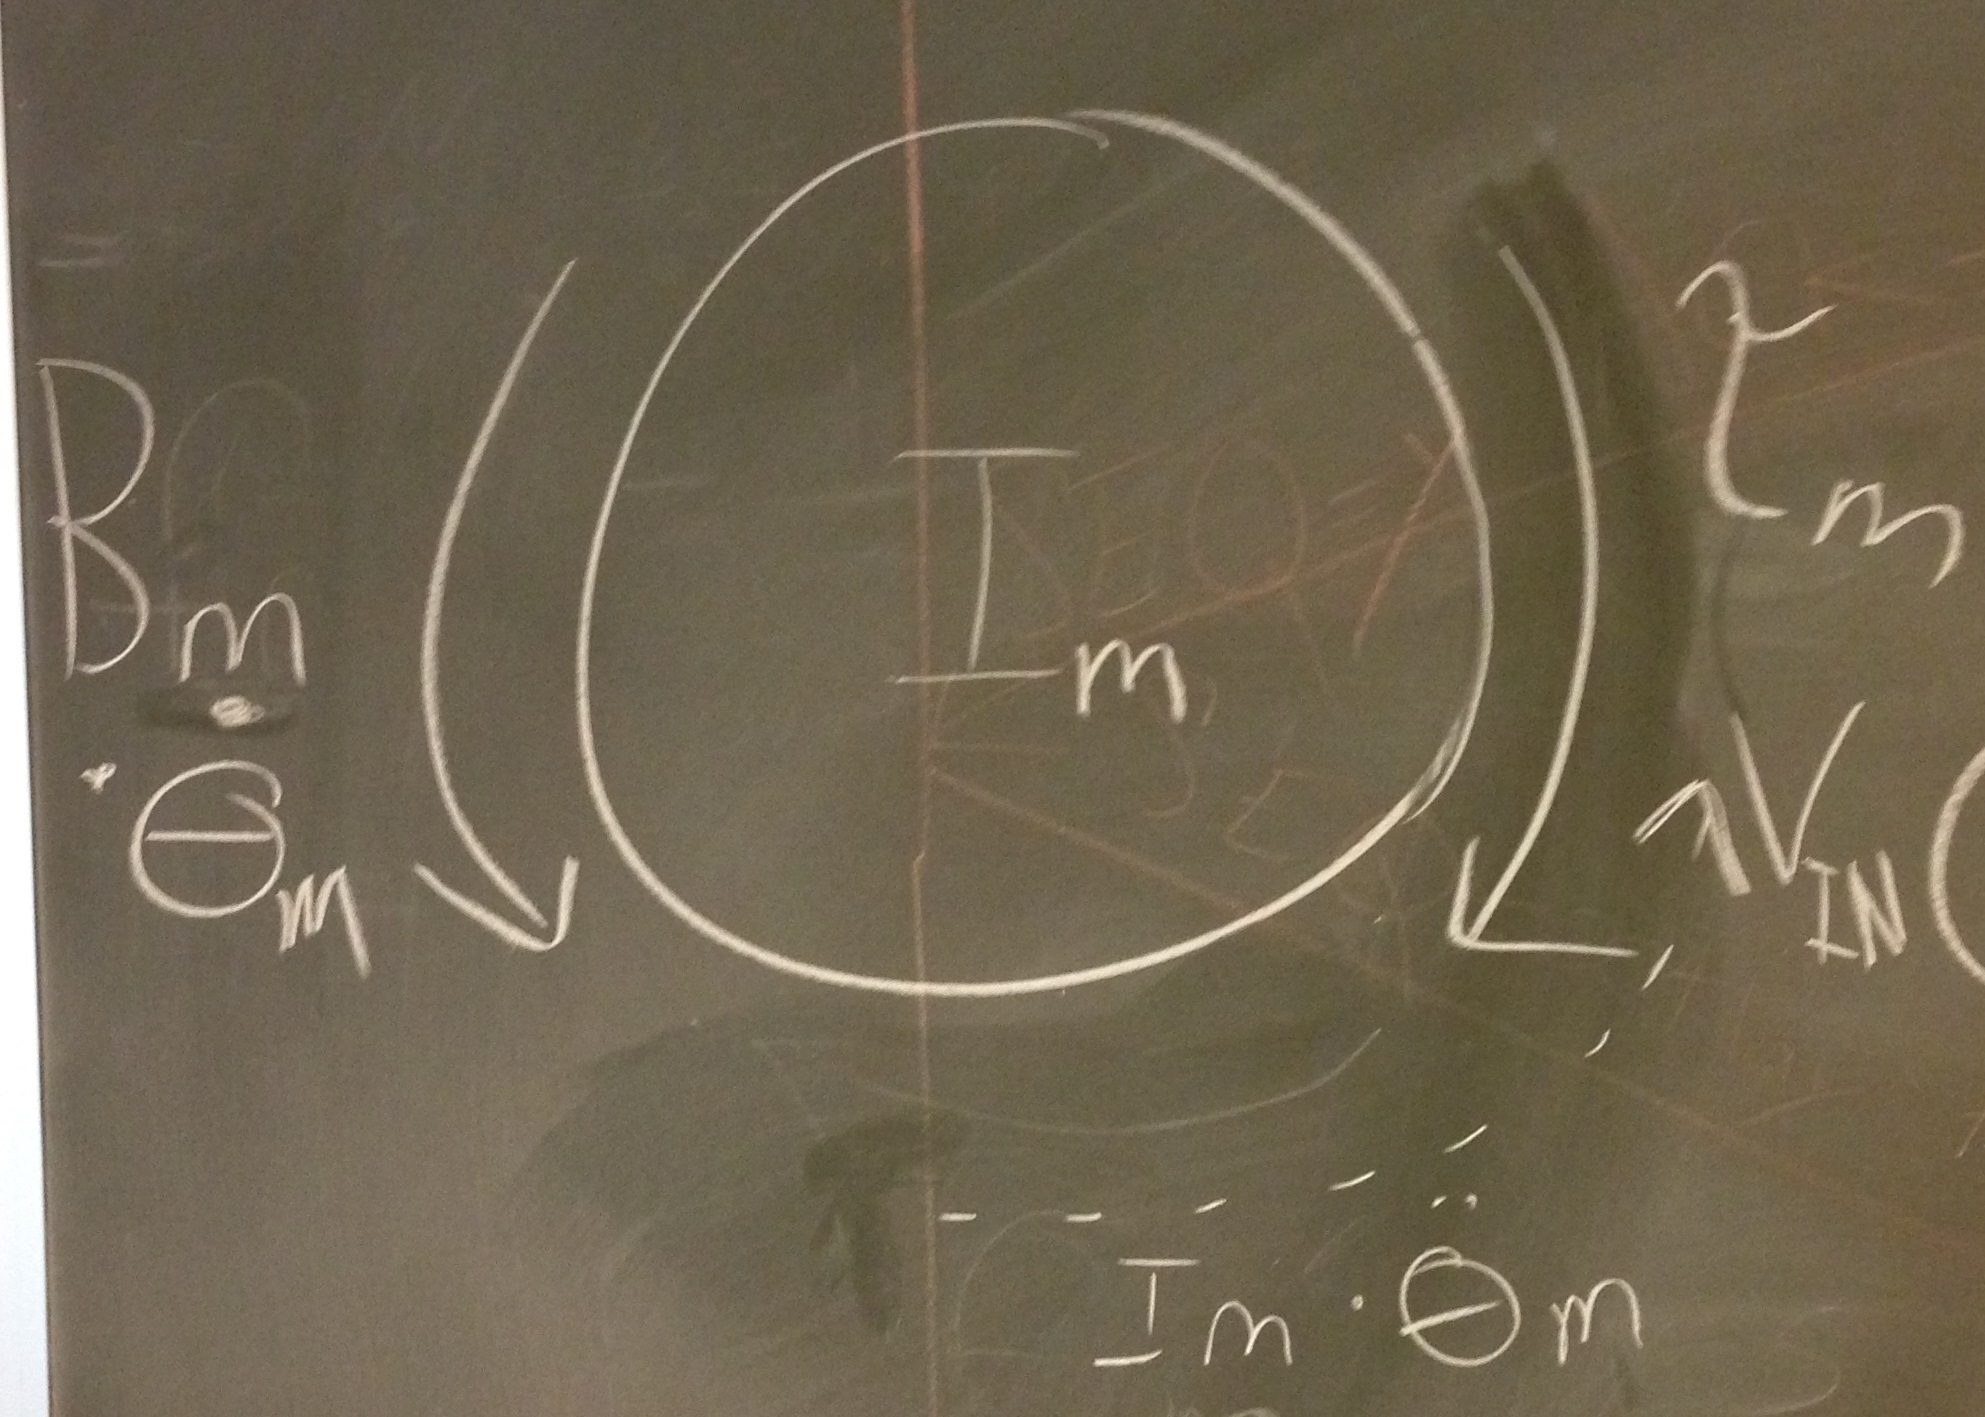
\includegraphics[width=\linewidth]{figures/MotorFreeBodyDiagram.jpg}
		\caption{Freebody diagram of the motor}
		\label{fig:MotorFreeBody}
	\end{subfigure}
	\caption{??}
	\label{fig:MotorElecFree}
\end{figure}

